\chapter{Eletricidade Cerebral}


\section{Correntes Elétricas}

\section{Neurônios}

\section{Impulsos Nervosos e Potencial de ação}


\section{Eletroencefalograma}


\section{Potenciais Relacionados a Eventos}


\section{Considerações Finais}

Impulsos nervosos são correntes elétricas emitidas pelos neurônios. Os neurônios são células responsáveis pela condução de impulsos nervosos que se comportam como um “cabo eletrificado” - 
analogia levantada no clássico estudo de Hodgkin e Huxley (1952). O conjunto de impulsos nervosos 
de grupos de neurônios geram campos magnéticos que 
podem ser captados por eletrodos colocados sobre a cabeça humana (Kandel, 2000). 
Estes campos magnéticos foram primeiro registrados de coletas em humanos aproximadamente em 1929,
 em um experimento conduzido pelo psiquiatra alemão Hans Berger (İnce et al., 2021) – figura 2.1. 
 Estes registros são o resultado dos potenciais de ação emitidos pelas células nervosas em proximidade ao eletrodo, e permitem uma boa resolução temporal do comportamento nervoso (podendo atingir precisão de milissegundos), mas em geral não permitem uma boa resolução espacial (como identificar a localização espacial do grupo celular responsável pela variação de voltagem observada). 


\begin{figure}[h]
    \centering
    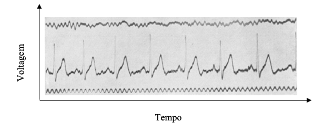
\includegraphics[width=100mm]{serie_temporal_EEG}
    \caption[Exemplo de um acelerador linear utilizado no Hospital Universitário de Brasília.]{Exemplo de um acelerador linear utilizado no Hospital Universitário de Brasília. Os ângulos de 360${^{\textrm{o}} }$, 180${^{\textrm{o}} }$ e 180${^{\textrm{o}} }$ indicam os possíveis valores de rotação do acelerador e do \emph{gantry}. Os valores em centímetros indicam as dimensões do \emph{gantry} e as distâncias em relação à mesa e ao chão. Fonte:~\cite{Avelino2013}.}\label{fig:acelerador}
    \end{figure}

A técnica de registro de EEG vem sendo desde então aperfeiçoada e escolhida 
em investigações comportamentais devido a sua natureza não invasiva.
Um exemplo de aperfeiçoamento foi a criação de um sistema internacional de posicionamentos 
de eletrodos para a coleta de EEG – o sistema 10/20 (Klem et al., 1999), 
representado na figura 2.2. O registro capturado nos eletrodos advém de uma 
diferença de potencial elétrico. Esta diferença pode ser em referência à um 
eletrodo colocado em uma região externa ao escalpo (como orelha), 
ou à uma voltagem média comum (Tavares, 2011).

\begin{figure}[h]
    \centering
    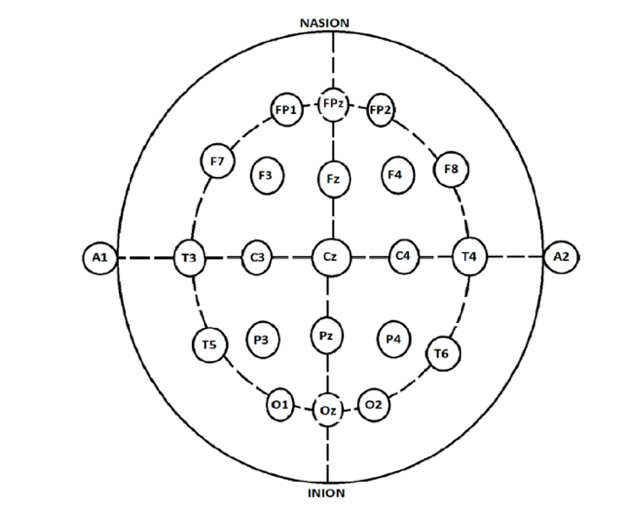
\includegraphics[width=100mm]{EEG_1020.png}
    \caption[Exemplo de um acelerador linear utilizado no Hospital Universitário de Brasília.]{Exemplo de um acelerador linear utilizado no Hospital Universitário de Brasília. Os ângulos de 360${^{\textrm{o}} }$, 180${^{\textrm{o}} }$ e 180${^{\textrm{o}} }$ indicam os possíveis valores de rotação do acelerador e do \emph{gantry}. Os valores em centímetros indicam as dimensões do \emph{gantry} e as distâncias em relação à mesa e ao chão. Fonte:~\cite{Avelino2013}.}\label{fig:acelerador}
    \end{figure}

\subsection{Tipos de Eletrodos para Captura de EEG}

Existem diferentes tipos de eletrodos para a captura de EEG. Um resumo é apresentado na tabela 2.1. É notável também que com o desenvolvimento da capacidade computacional, novos recursos e métodos para a análise destes dados vem sendo benéficos à construção do conhecimento científico, agora também contando com o desenvolvimento de algoritmos de aprendizado de máquina, aprendizado profundo e inteligência artificial. 